\section{Improving HuMoR TestOps}
\label{sec:humor_improvement}

This section presents the attempt that was made at modifying the TestOps procedure in such a way that we attain comparable results but in a significantly shorter time.

\subsection{Speeding up the TestOps}
\label{sec:humor_improvement_speed}

Realising that the main speed limitations are due to the concept of rollout over the entire sequence, we decided to break this long-range dependence. Through short overlapping rollouts, it is possible to achieve more parallelisation and smaller computation graphs, and our intuition suggested that there is no need for such a large context window, that only a small number of autoregressed frames are needed to be able to propagate information sensibly and to get meaningful gradients. Anecdotally, it would seem intuitive that if a video contains sitting, then walking, then sitting again, the second act of sitting would not depend on the early act of sitting, hence rolling out over the whole sequence seems unnecessary.

The HuMoR TestOps rollout is presented graphically in \figref{fig:humor_rollout_graph}. To begin with \textbf{all} the states are autoregressed from the initial state and the latent variables, and only then are the losses applied. This results in very long-range dependencies in the computation graph, thus making the gradients time-consuming to calculate. 

\begin{figure}
    \centering
    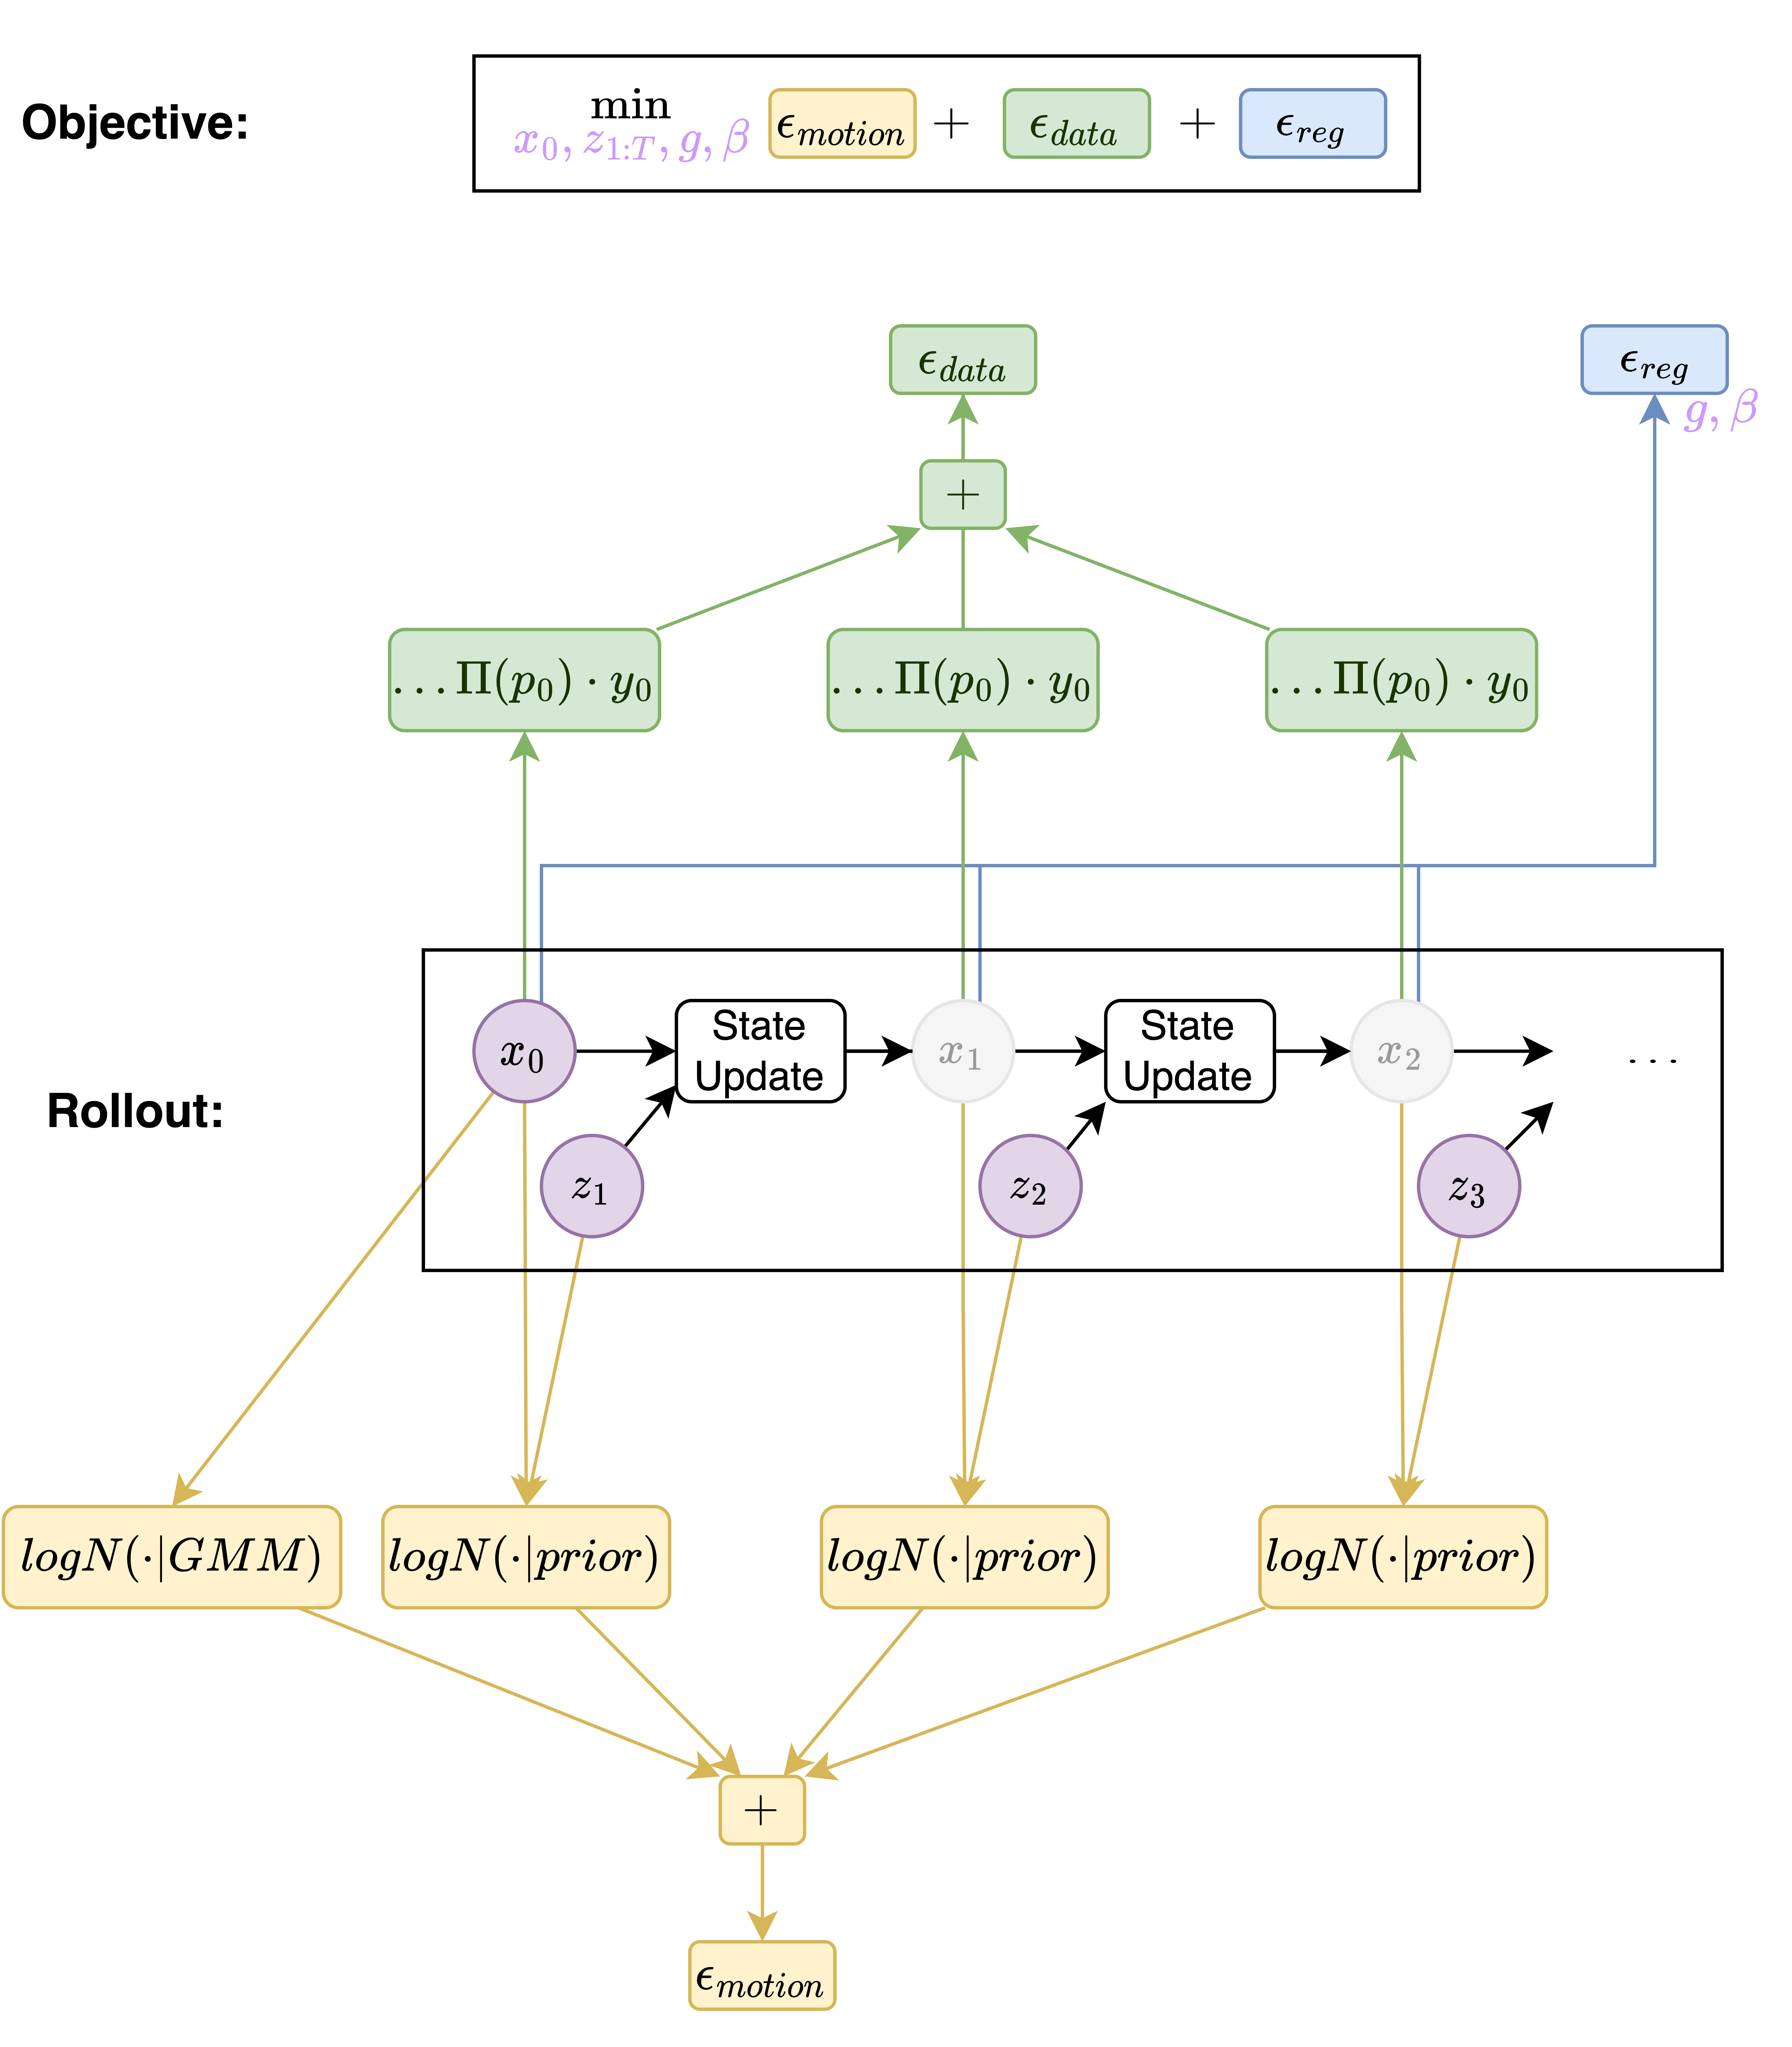
\includegraphics[width=1\textwidth]{Figures/humor/improvement/computation_graph_humor.png}
    \caption{TestOps Stage 3 Computation Graph}
    \label{fig:humor_rollout_graph}
    \medskip
    \small
    \raggedright
    The optimised variables are highlighted in purple, $\mathbf{x}$ being the state (root, joint positions etc.), and $\mathbf{z}$ the latent transitions. The gray $\mathbf{x}$'s indicate the states that are calculated during the rollout (c.f \secref{sec:humor_test_ops}) and the losses that are applied after the rollout are color coded. $\textcolor{Goldenrod}{\epsilon_{motion}}$ is the loss due to the HuMoR prior (and initial state likelihood GMM briefly mentioned in \secref{sec:humor_testops_extra_notes}). $\textcolor{ForestGreen}{\epsilon_{data}}$ is the projection loss comparing the projected state to the OpenPose predictions. $\textcolor{RoyalBlue}{\epsilon_{reg}}$ are the regularisation losses, smoothness, foot contacts, etc (and are also the losses responsible for the ground plane $g$ and the shape parameters $\beta$ briefly mentioned in \secref{sec:humor_testops_extra_notes}). The 'State Update' node represents the application of the HuMoR decoder to the previous state and latent transition to obtain a pose update, and the application of this pose update to obtain a new pose.
\end{figure}

The most obvious way to break this autoregression is to maintain a separate persistent sequence of states, $\mathbf{x}_{1:T}$, updating these with reference to the states decoded from the latent variables. We could take into account the decoded states, $\mathbf{x'}_{1:T}$, in several manners (using optimisation techniques or direct updates):
\begin{enumerate}
    \item Copy over
    \begin{itemize}
        \item Directly replace the persistent sequence of $\mathbf{x}_{1:T}$ with the decoded sequence $\mathbf{x'}_{1:T}$.
    \end{itemize}
    \item Blend
    \begin{itemize}
        \item Perform a weighted addition of the persistent $\mathbf{x}_{1:T}$ and decoded $\mathbf{x'}_{1:T}$.
    \end{itemize}
    \item Loss term
    \begin{itemize}
        \item Add a loss term on the difference between the persistent $\mathbf{x}_{1:T}$ and decoded $\mathbf{x'}_{1:T}$. 
    \end{itemize}
\end{enumerate}

In \figref{fig:dimm_rollout_graph} we can see the example of adding a loss term on the difference between the persistent $\mathbf{x}_{1:T}$ and decoded $\mathbf{x'}_{1:T}$.

The motivation behind this change is the idea that all decoding steps can now be performed in parallel, rather than sequentially, which greatly reduces the compute time. The maintaining of a persistent sequence of states, $\mathbf{x}_{1:T}$, allows for the information to flow forwards through the short-range rollouts, and over the iterations of the optimiser. Note however that the information flow will be slower than the HuMoR TestOps, as in the TestOps all subsequent $\mathbf{x}$'s are regressed from the initial $\mathbf{x}_0$ and thus the chain is unbroken from beginning to end of the sequence every single rollout (though as discussed in \secref{sec:humor_improvement_speed} we don't believe this to be necessary). In the HuMoR TestOps information can flow backward from any future frame $\mathbf{x}_t$, as the computation graph links all the states through the auto-regression, in the new method however, the information flow will be much more limited, as the rollouts will be significantly shorter, though the information can still flow through the iterations of the optimiser.

\begin{figure}
    \centering
    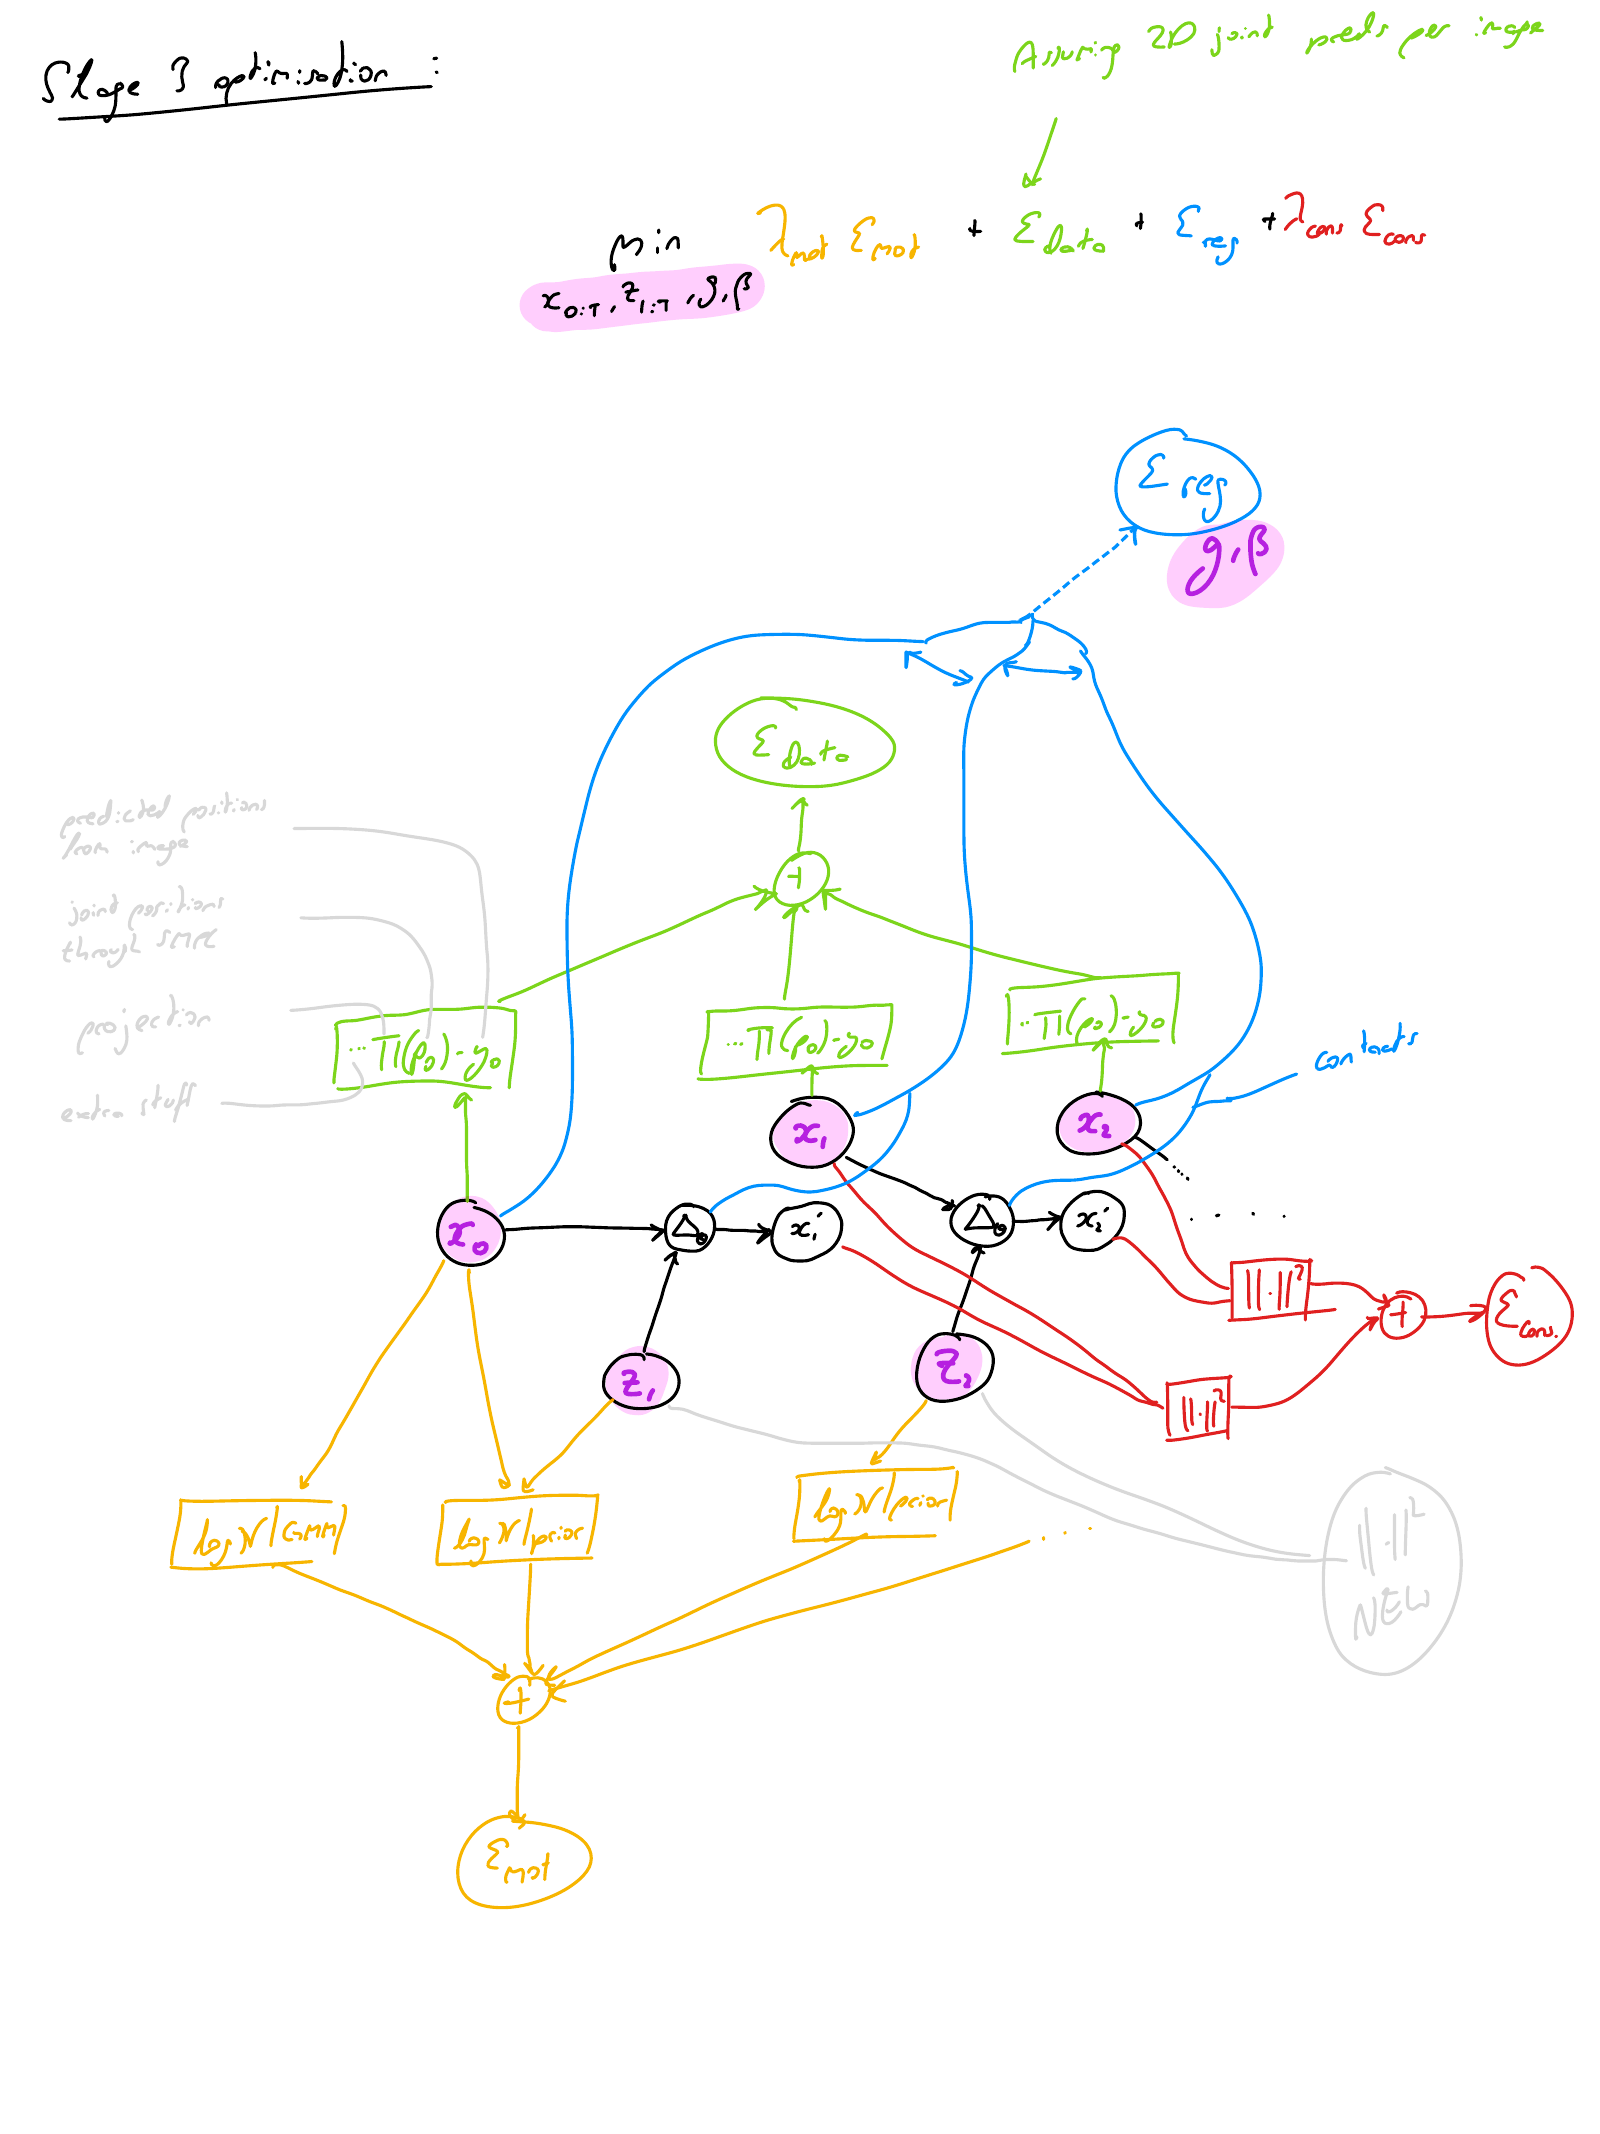
\includegraphics[width=1\textwidth]{Figures/humor/improvement/computation_graph_dimm.png}
    \caption{Decoupled Computation Graph}
    \label{fig:dimm_rollout_graph}
    \medskip
    \small
    \raggedright
    The computation graph is similar to that presented in \figref{fig:dimm_rollout_graph}. This time however we roll out one step, maintain a persistent sequence of states, $\textcolor{Mulberry}{\mathbf{x}_{1:T}}$, and add a loss term, $\textcolor{Red}{\epsilon_{consistency}}$ on the difference between the persistent $\textcolor{Mulberry}{\mathbf{x}_{1:T}}$ and decoded $\textcolor{Gray}{\mathbf{x'}_{1:T}}$. This theoretically allows for parallelised decoding of the latent variables, and thus a much faster computation time, by avoiding the rollout and large computation graph.
\end{figure}

This new formulation also allows us to experiment with different degrees of rollout. We can once again decode the decoded sequence of $\mathbf{x'}$'s to get $\mathbf{x''}$, and so on and so forth. These extra sequences are all decoded with the same latent variables thus the updates to the latent variables will take into account the losses on all the decoded sequences. Graphically this can be seen in \figref{fig:dimm_decoded_sequences}, where each next line is a newly decoded sequence derived from the previous.

\begin{figure}
    \centering
    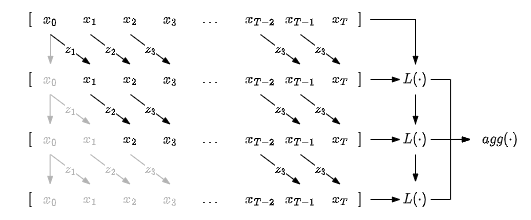
\includegraphics[width=1\textwidth]{Figures/humor/improvement/Rollout_overlap.png}
    \caption{Decoded sequences}
    \label{fig:dimm_decoded_sequences}
    \medskip
    \small
    \raggedright
    The formulation of the optimisation problem shown in \figref{fig:dimm_rollout_graph} can be extended by further rollout. Each time we can reapply the latent variables $\mathbf{z}_{1:T}$ to obtain a new sequence. In applying losses to these sequences, we can update the latent variables taking into account all the decoded sequences, thus can more quickly propagate information backward through the introduction of a limited rollout. Note that the grayed-out variables are redundant and hence ignored.
\end{figure}





\subsection{Implementation notes}

A number of issues were encountered during the implementation that are worth mentioning. After implementing the new method, attempts were made to get the optimiser to produce sensible results. The general approach was to use a small number of losses, so as to get a better intuition of each loss, with the goal of better understanding how to balance the losses in the optimiser, but some errors in individual losses were encountered.

Firstly, as expected, the Axis-Angle representation became a problem. When running through functions to convert to root-local reference frame for the HuMoR model decoder (as it operates on said reference frame), and then back to world reference frame for the optimiser, the Axis-Angle vector flipped direction. Though the flipped vector still represented the same rotation, the numerical values of the axis angle representations in the persistent sequence of $\mathbf{x}_{0:T}$ and the decoded sequence of $\mathbf{x}_{0:T}$ were now different, hence incorporating the information from the decoded sequence in the persistent sequence caused the angle to find a middle point between the flipped values which was no longer a sensible angle representation, thus resulting in strange rotations and artifacts in the final sequence. We mitigated this issue by optimising in 6d rotation representation.

Secondly, an issue in the SMPL model was found. When using a 2d reprojection loss (comparing the projected joints to the OpenPose 2d predictions) on a sequence where only the left arm and face had any OpenPose predictions, the legs were being moved by the optimiser. This seemed dubious as the losses were only seeing the arm and face joints, hence no gradients should have flowed to the legs. It was eventually found that the skinning weights of the SMPL model \cite{SMPL} contain spurious long-range connections. 3\% of the LBS (linear blend skinning) weights in the SMPL model are non-zero but less than $1e-2$, which seems rather too low to have any meaningful effect on the skinning, but which allows for spurious gradients to flow. For example, the vertex 332 of the SMPL mesh \cite{SMPL_op_joints}, representing the nose joint which we need for a comparison to the OpenPose skeleton, is skinned $99.8\%$ by the 'head' joint, but also spuriously $0.2\%$ by the right hip, left knee and right knee. This issue was solved by pruning all weights below 1e-2. It is interesting to note that there are known spurious connections in the SMPL blend shapes \cite{STAR}, but that we have found no reference to spurious connections in the LBS weights. 
\\
% For the projection loss where a comparison to the OpenPose predictions is necessary, the OpenPose skeleton must be obtained from the SMPL mesh parametrized by the state $\mathbf{x}_{1:T}$. Certain joints are regressed from the SMPL mesh (see \cite{SMPL} for more details), other are simply taken directly as vertices from the mesh, as is the case for the nose joint in the OpenPose skeleton which is taken to be vertex 332 \cite{SMPL_op_joints}. We noted that this vertex 332 is skinned $99.8\%$ by the 'head' joint, but also spuriously $0.2\%$ by the right hip, left knee and right knee. This issue was solved by pruning all weights below 1e-2. It is interesting to note that there are known spurious connections in the SMPL blend shapes \cite{STAR}, but that we have found no reference to spurious connections in the LBS weights.













\subsection{Experiments}

\subsubsection{Initial $\mathbf{z}_{1:T}$}
To begin with, we looked into the initial $\mathbf{z}_{1:T}$ that was obtained from projecting the Stage 2 $\mathbf{x}_{0:T}$ through the HuMoR encoder. We found that in occluded situations this $\mathbf{z}_{1:T}$ already encodes a sitting motion when locally rolled out, as seen in \figref{fig:humor_stage_2_rollout_sitting}, thus $\mathbf{z}_{1:T}$ represents a meaningful starting point for the Stage 3 optimisation. We note however that when we perform a longer rollout the resultant motion sequence, shown in \figref{fig:humor_stage_2_rollout_deviation}, deviates largely from the initial sequence $\mathbf{x}_{0:T}$ seen in \figref{fig:humor_stage_2}.
This shows us that though the initial $\mathbf{z}_{1:T}$ encodes some sensible motion locally and though they can be used to accurately recover the next frame, when they are chained together small errors accumulate to create an overall divergence. For example, if the arm is moved slightly too much by a single $\mathbf{z}_t$, then all the future frames will have the arm in slightly the wrong position, and if multiple latent variables $\mathbf{z}_{t:t'}$ are wrong in the same direction, then the arm will raise up. 

% This diverging sequence is the initial point for Stage 3 of the HuMoR TestOps in which the rollout is optimised, and it seems unfortunate to us that from a sensible starting sequence $\mathbf{x}_{0:T}$ obtained from Stage 2 we get such a bad initial sequence. We do however note that while this starting point represents a sequence that diverges heavily, the $\mathbf{z}_{1:T}$ might not need to move so far to avoid such accumulation effects. The intuition that motivates our formulation is the fact that we are not completely throwing out the sensible starting point $\mathbf{x}_{0:T}$ and $\mathbf{z}_{1:T}$ obtained from Stage 2, and therefore that it should be possible to refine the $\mathbf{x}_{0:T}$ by taking into account the HuMoR model through the $\mathbf{z}_{1:T}$ whilst updating the $\mathbf{z}_{1:T}$ in a more efficient manner than simply discarding these $\mathbf{x}_{0:T}$ through an initial rollout.

\begin{figure}
    \centering
    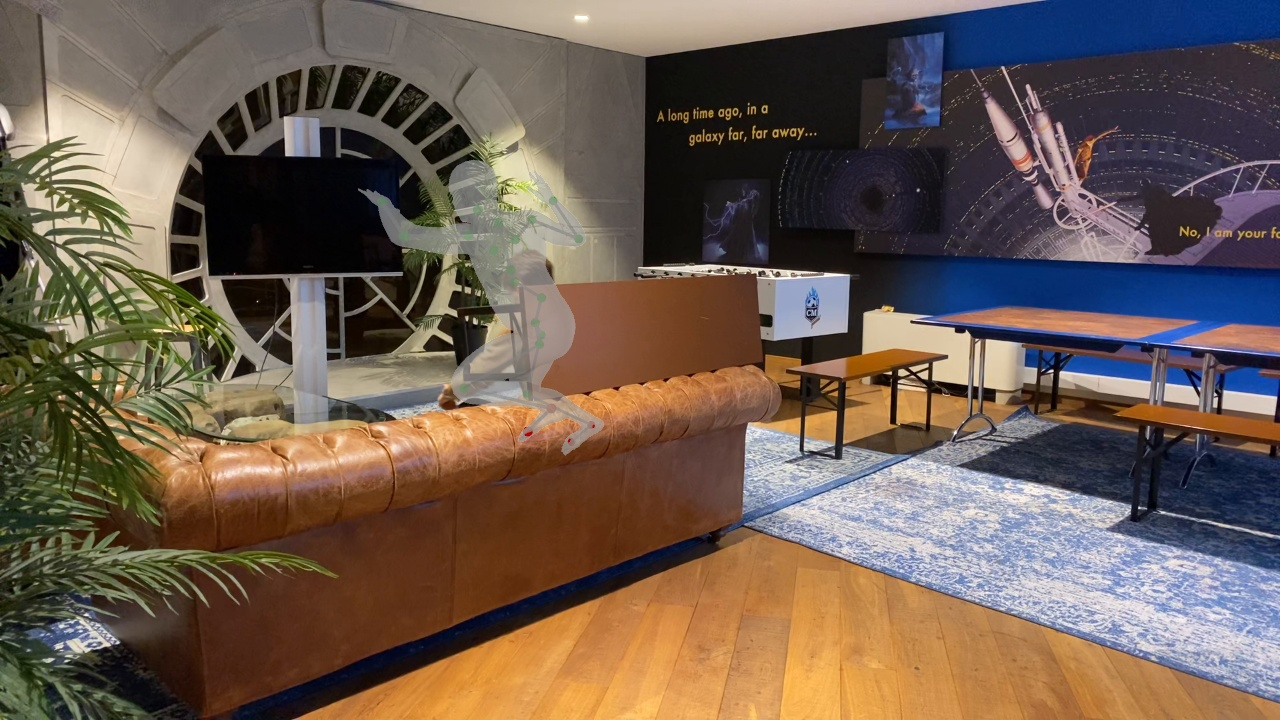
\includegraphics[width=1\textwidth]{Figures/humor/improvement/Rollout_stage_2/sitting_clip/rollout_sitting_example/frame_00000078.jpg}
    \caption{Stage 2 $\mathbf{z}_{1:T}$ encode a sitting motion}
    \label{fig:humor_stage_2_rollout_sitting}
    \medskip
    \small
    \raggedright
    Here we can see that the legs bend in a sitting/squatting motion. The arms raising are due to an accumulation of errors. 
\end{figure}

\begin{figure}
    \centering
    \subfloat[]{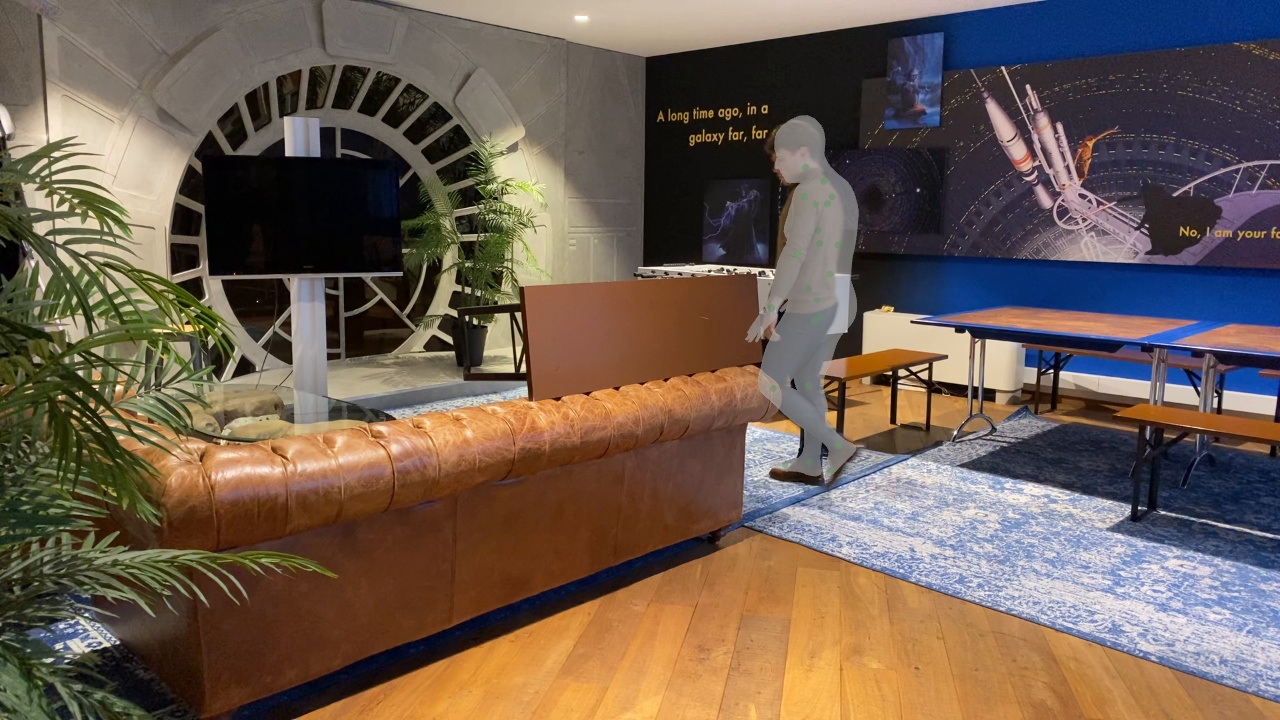
\includegraphics[width=0.3\textwidth]{Figures/humor/improvement/Rollout_stage_2/sitting_clip/stage2/frame_00000099.jpg}} 
    \hfil
    \subfloat[]{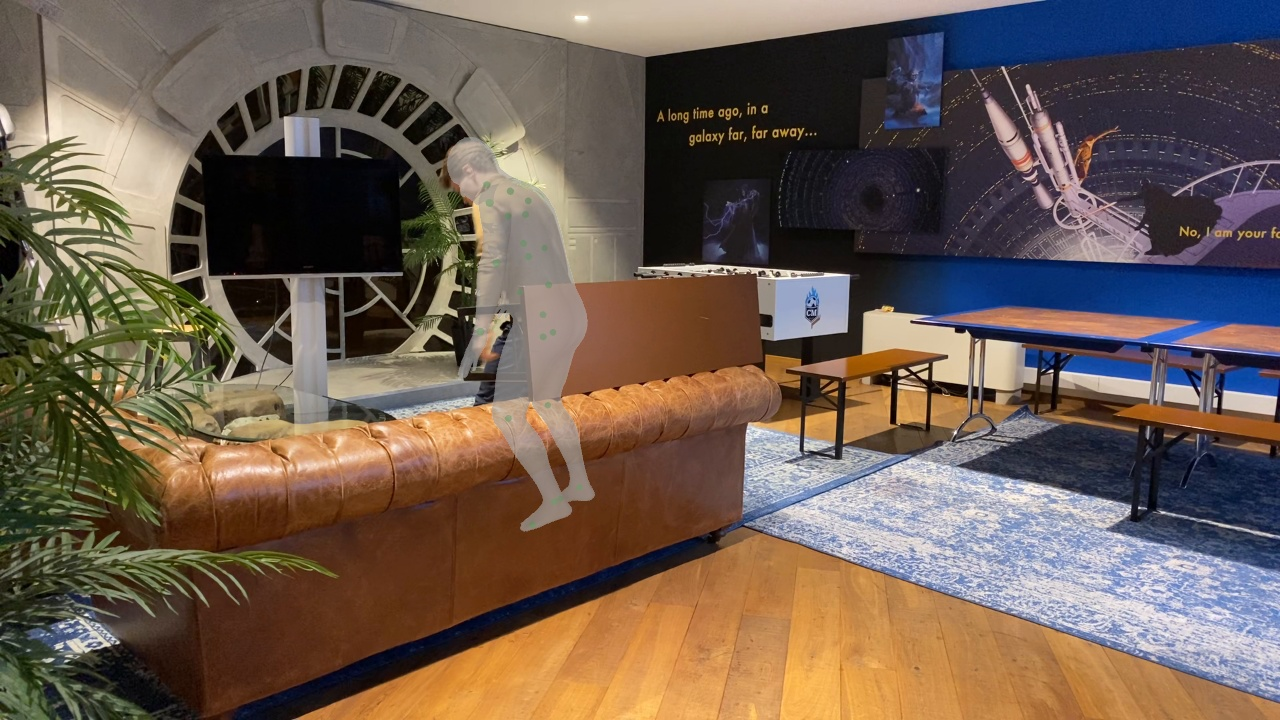
\includegraphics[width=0.3\textwidth]{Figures/humor/improvement/Rollout_stage_2/sitting_clip/stage2/frame_00000149.jpg}} 
    \hfil
    \subfloat[]{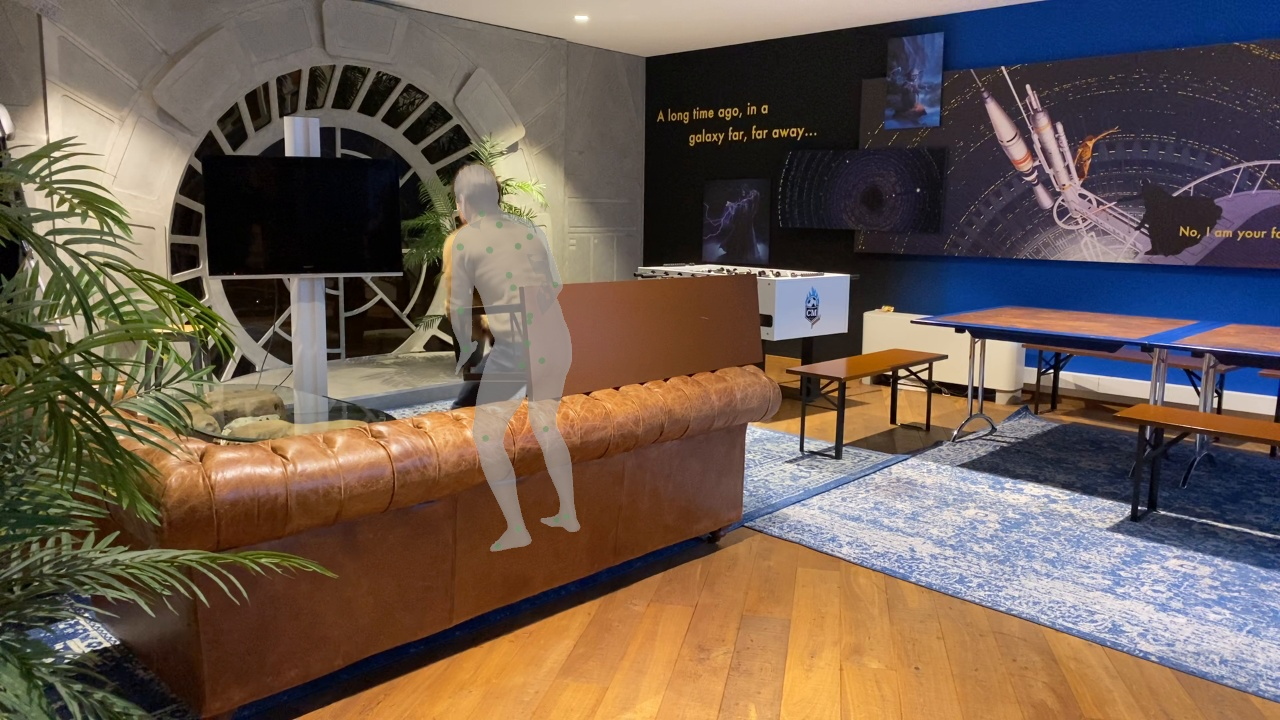
\includegraphics[width=0.3\textwidth]{Figures/humor/improvement/Rollout_stage_2/sitting_clip/stage2/frame_00000219.jpg}}
    \hfil
    \subfloat[]{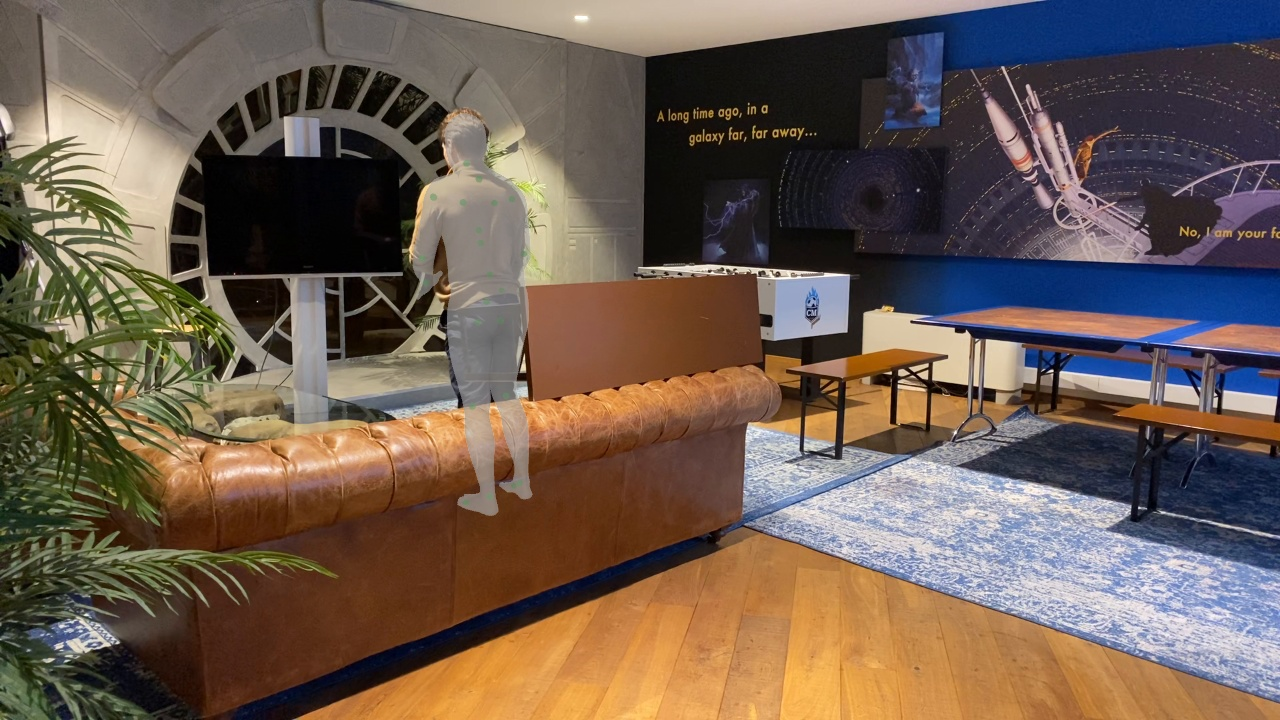
\includegraphics[width=0.3\textwidth]{Figures/humor/improvement/Rollout_stage_2/sitting_clip/stage2/frame_00000239.jpg}}
    \caption{Stage 2 $\mathbf{x}_{0:T}$}
    \label{fig:humor_stage_2}
\end{figure}

\begin{figure}
    \centering
    \subfloat[]{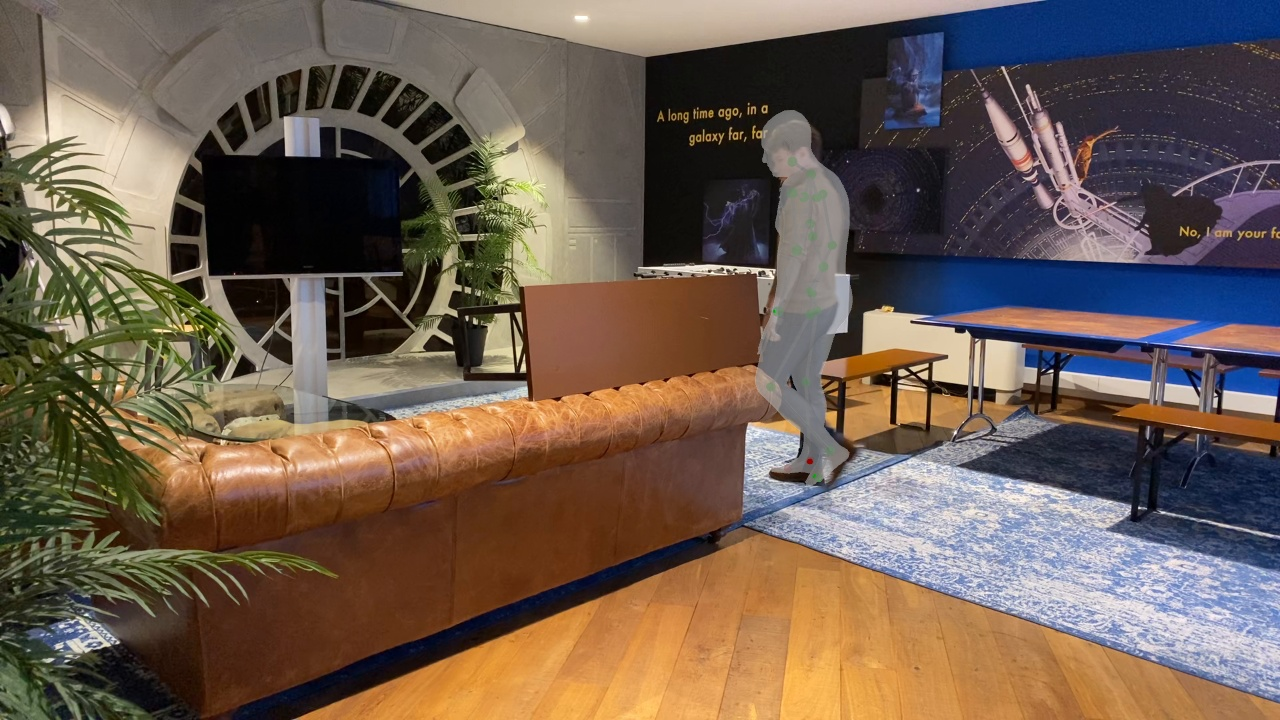
\includegraphics[width=0.3\textwidth]{Figures/humor/improvement/Rollout_stage_2/sitting_clip/rollout/frame_00000010.jpg}} 
    \hfil
    \subfloat[]{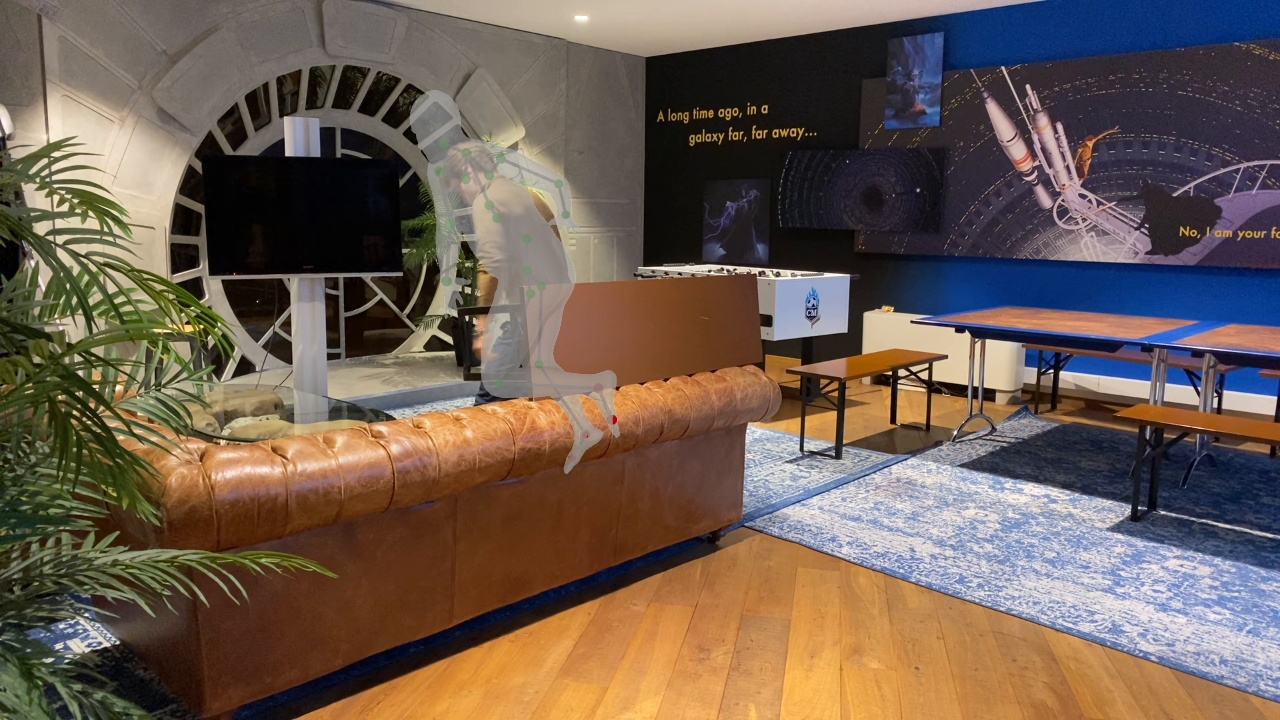
\includegraphics[width=0.3\textwidth]{Figures/humor/improvement/Rollout_stage_2/sitting_clip/rollout/frame_00000060.jpg}} 
    \hfil
    \subfloat[]{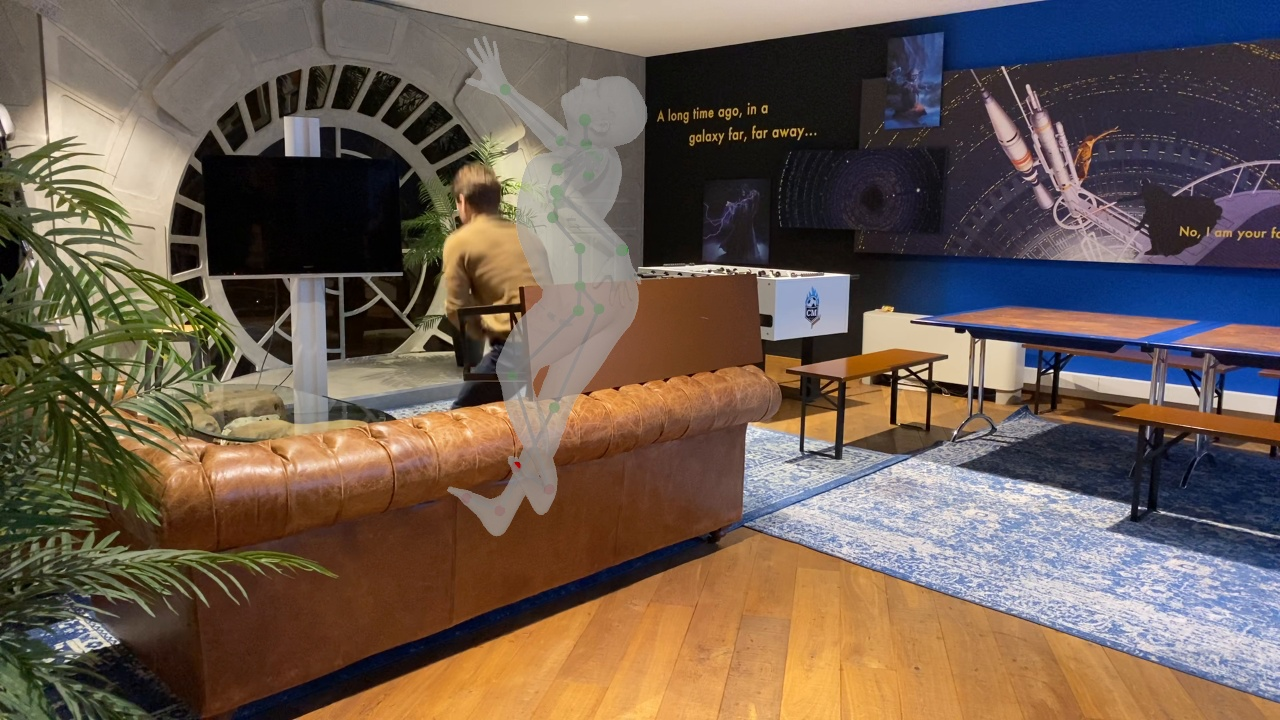
\includegraphics[width=0.3\textwidth]{Figures/humor/improvement/Rollout_stage_2/sitting_clip/rollout/frame_00000130.jpg}}
    \hfil
    \subfloat[]{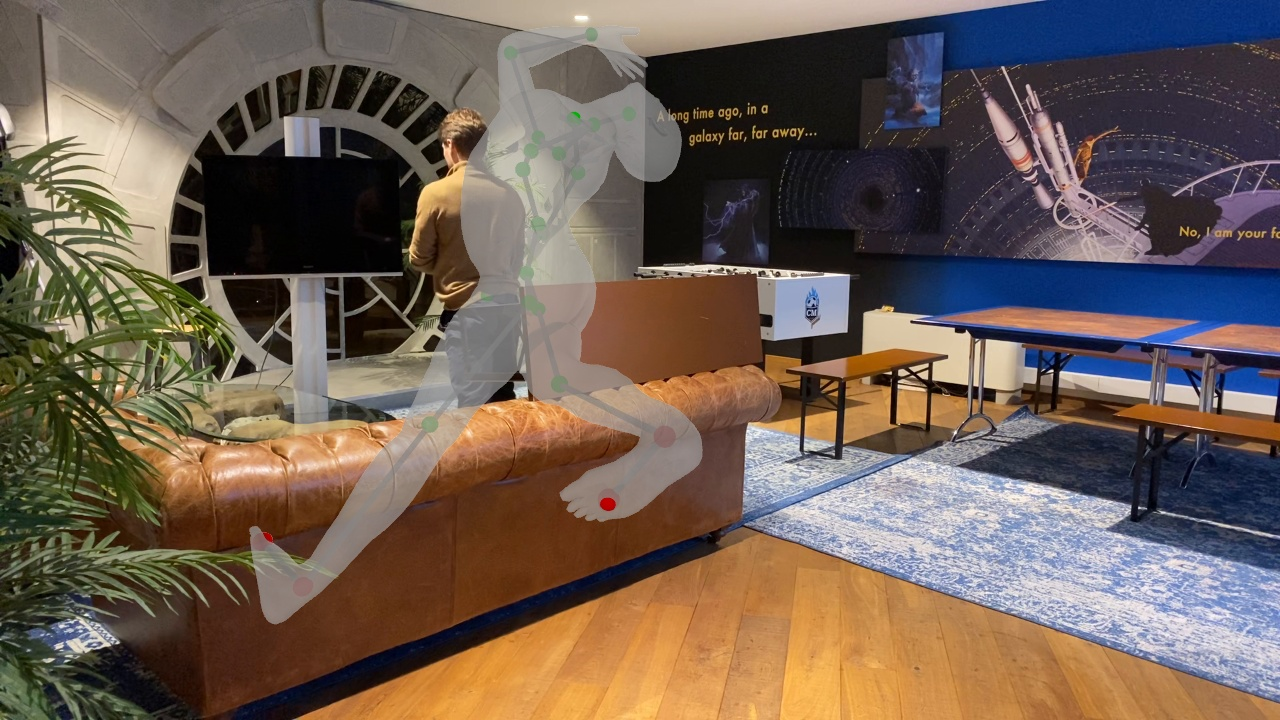
\includegraphics[width=0.3\textwidth]{Figures/humor/improvement/Rollout_stage_2/sitting_clip/rollout/frame_00000150.jpg}}
    \caption{Deviation due to rollout of Stage 2 $\mathbf{z}_{1:T}$}
    \label{fig:humor_stage_2_rollout_deviation}
\end{figure}

Armed with this understanding of the starting point of our optimisation variables, we moved on to attempting to optimise them. We note that the next experiments were performed with varying numbers of decoding steps, 1, 2, 5, and 10, and that we found that longer rollouts produced more stable results but at the cost of longer compute times, as intuition would suggest.


\subsubsection{Jointly optimising $\mathbf{x}_{0:T}$ and $\mathbf{z}_{1:T}$}
\label{sec:humor_experiments_jointly_optimising}
Next, we embarked upon some preliminary experimentation in which we began optimising $\mathbf{x}_{0:T}$ and $\mathbf{z}_{1:T}$. We found that the most successful approach to blending the decoded and persistent  $\mathbf{x}_{1:T}$ among those described in \secref{sec:humor_improvement_speed} was to have an L1 loss on the difference between them. We saw that when simply copying over, the propagation of small errors forward was too strong (the effect shown in \figref{fig:humor_stage_2_rollout_deviation}) and the system failed to recover as it no longer had access to the long-range gradients present in the HuMoR TestOps method rollout. We also found that when blending rather than completely copying over that the weighting of the blending was another parameter that was difficult to choose. Hence having a loss was the best method.

We then experimented with jointly optimising $\mathbf{x}_{0:T}$ and $\mathbf{z}_{1:T}$ with a larger variety of losses. It was noted that the sitting down motion was not achieved consistently. However as previously mentioned, the initial $\mathbf{z}_{1:T}$ encode a sitting motion, thus we conject that the $\mathbf{x}_{0:T}$ and $\mathbf{z}_{1:T}$ were fighting and this sitting motion was lost, that is to say, the $\mathbf{z}_{1:T}$ move to match the initial $\mathbf{x}_{0:T}$ motion in which the skeleton simply clips into the floor without bending the legs, thus the $\mathbf{z}_{1:T}$ begin encoding less leg bending. To avoid this issue in future experiments, the $\mathbf{z}_{1:T}$ were detached from the consistency loss that encourages the persistent $\mathbf{x}_{0:T}$ match the decoded $\mathbf{x}_{0:T}$.

These experiments allowed us to choose a blending strategy for the decoded and persistent $\mathbf{x}_{0:T}$, and indicated that jointly optimising $\mathbf{x}_{0:T}$ and $\mathbf{z}_{1:T}$ was a difficult task due to divergent goals and difficult balancing, thereby suggesting we try optimising them separately.

\subsubsection{Separately optimising $\mathbf{x}_{0:T}$ and $\mathbf{z}_{1:T}$}
We next embarked upon some experiments in which the goal was either to optimise $\mathbf{x}_{0:T}$ whilst keeping $\mathbf{z}_{1:T}$ fixed or vice versa, so as to avoid the divergent goals found in \secref{sec:humor_experiments_jointly_optimising} and to see if information could be passed between latent transitions and poses sensibly.

With the $\mathbf{z}_{1:T}$ fixed at their initial state and after considerable effort to balance the optimiser, we managed to achieve a sensible sitting motion for a clip containing occluded sitting, however when we applied the same optimiser settings to a longer clip the results were no longer satisfactory. We also noted that when it did work, it required a large number of iterations, in the 1000s, which took 10mins or more, thus the speedup was not as evident as hoped.

In the inverse case consisting of fixing $\mathbf{x}_{0:T}$ to the final HuMoR optimised states and optimising $\mathbf{z}_{1:T}$, we noted that we consistently converge in the direction of the final HuMoR $\mathbf{z}_{1:T}$ states, which indicates that we are optimising in a sensible direction.

\begin{figure}
    \centering
    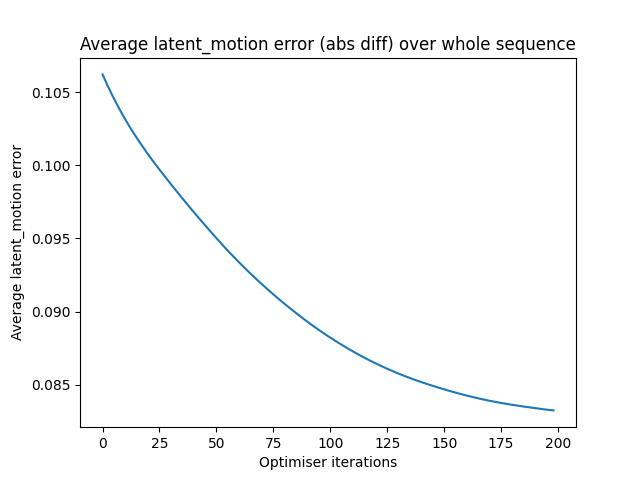
\includegraphics[width=0.75\textwidth]{Figures/humor/experiments/avg_latent_motion_error.png}
    \caption{Optimising $\mathbf{z}_{1:T}$ with fixed $\mathbf{x}_{0:T}$}
    \label{fig:zs_converge_to_humor_zs}
    \medskip
    \small
    \raggedright
    With $\mathbf{x}_{0:T}$ fixed to be the final HuMoR TestOps solution, we found that the $\mathbf{z}_{1:T}$ converges in the direction of the $\mathbf{z}_{1:T}^{(HuMoR)}$ found by the HuMoR TestOps ('latent\_motion error' is the average absolute difference between these quantities). This indicates that our method also considers the HuMoR solution to be sensible, and gives us hope that it is possible to arrive at the same solution with a faster method.
\end{figure}

These experiments showed that the information can be passed sensibly from $\mathbf{x}_{0:T}$ to $\mathbf{z}_{1:T}$ and vice versa, however that this was no easy task.

\subsubsection{Next step}
The previous experiments all suggest that the next direction to pursue would be an optimisation scheme in which we go back and forth between optimising $\mathbf{z}_{1:T}$ then $\mathbf{x}_{0:T}$. This would avoid the competing goals and difficult to balance optimiser we found when jointly optimising $\mathbf{z}_{1:T}$ and $\mathbf{x}_{0:T}$, and would allow further exploration of the promising results found when optimising $\mathbf{z}_{1:T}$ and $\mathbf{x}_{0:T}$ separately. However considering our difficulty in achieving consistent results for the optimisation of $\mathbf{x}_{0:T}$ with fixed $\mathbf{z}_{1:T}$, our ever growing feeling that this method was not the most efficient formulation of the problem, my desire to try a new direction, and the time constraints, we deemed it time to move on and investigate a new method.


\subsection{Improvement Conclusion}

We found that jointly optimising the $\mathbf{x}_{0:T}$ and $\mathbf{z}_{1:T}$ did not prove an easy task to solve, which may indicate that
\begin{itemize}
    \item it is a particularly difficult problem, and therefore that the optimiser struggles to satisfy the constraints and find a good minimum for both $\mathbf{x}$ and $\mathbf{z}$ at the same time
    \item the coupling of the $\mathbf{x}_{0:T}$ and $\mathbf{z}_{1:T}$ in the HuMoR decoder is an important issue. We found it to be at the very least a minor issue as it was necessary to decouple the $\mathbf{z}_{1:T}$ from the consistency loss (matching the persistent $\mathbf{x}_{1:T}$ to the decoded $\mathbf{x'}_{1:T}$) to avoid the $\mathbf{z}_{1:T}$ being modified in such a way as to fit the unoptimised $\mathbf{x}_{0:T}$ at the beginning of the optimisation schedule
    \item the optimiser is badly balanced
\end{itemize}
This suggests that a new decoder that does not couple $\mathbf{x}_{0:T}$ and $\mathbf{z}_{1:T}$ would be useful and worth investigating if a similar method is pursued in the future.

In the investigations, we found it possible to achieve sensible results on a given clip when optimising either the $\mathbf{x}_{0:T}$ or the $\mathbf{z}_{1:T}$ separately. For example fixing the unoptimised initial $\mathbf{z}_{1:T}$, we produce a plausible sitting motion in a short occluded sequence. However, we find that the same settings for the optimiser failed to achieve a good result on an alternative clip. This may indicate that 
\begin{itemize}
    \item again, this is a difficult problem that the optimiser will struggle to solve
    \item the optimiser is badly balanced
\end{itemize} as before.

While many of the issues encountered may simply be due to a badly balanced optimiser, considerable effort was made to mitigate this potential issue, and therefore it is our impression that this problem is at the very least a tricky one in the formulation we were investigating. This investigation did not result in a better model, however allowed us to improve our intuition, understand and fix several issues, and gain more insight into the problem and how best to achieve our goals. We therefore can make a more informed decision with respect to which direction to pursue next. \\
We found that taking a system that was designed with autoregression in mind and trying to parrallelise it, proved more difficult than expected. The experiments lead us to believe that jointly optimising a sequence of poses and latent variables obtained through a single frame decoder may be a more difficult formulation of the problem than necessary. We therefore conclude that a method in which we model longer motion sequences may be more fruitful.